\documentclass[11pt]{article}

\title{\textbf{Project CS 2012\\Course Report}}
\author{Paolo Boschini\\
		Thiago Costa Porto\\
		Harold Martinez\\
		Linus Sunde\\
		Kim-Anh Tran}
\date{}

% usepackage
\usepackage{graphicx}
\usepackage{parskip}
\usepackage{hyperref}

% new commands and environments
\newenvironment{myindentpar}[1]%
 {\begin{list}{}%
         {\setlength{\leftmargin}{#1}}%
         \item[]%
 }
 {\end{list}}
 
 % References
\newcommand{\fig}[1]{Figure ~\ref{fig:#1}}
\newcommand{\tab}[1]{Table ~\ref{tab:#1}}
\newcommand{\sect}[1]{Section ~\ref{sec:#1}}
 
% other
\parskip 12pt
\parindent 0pt

\begin{document}

\maketitle

\section{Git and Jenkins}
For our project we have decided to choose Git as a version
control system and Jenkins as a continuous integration tool. 
The following sections will describe our approach of using
both tools for our development.

\subsection{Creating, sharing,  and deleting a branch}
Each time we want to add new code to our current project,
we need to create a new branch:

\begin{myindentpar}{3cm}
git checkout -b my\_own\_branch
\end{myindentpar}

On my\_own\_branch we only commit changes as long
as this branch is not shared. 

In case we want to share a particular branch with 
another person, we need to push it:

\begin{myindentpar}{3cm}
git push origin shared\_branch
\end{myindentpar}

As soon as we work on a branch that is shared between
several people, our convention to submit code is the following:

\begin{enumerate}
 \item \textbf{Commit} your changes
 \item \textbf{Pull} changes from other people
 \item \textbf{Push} your changes
\end{enumerate}

In order to delete branches that are local, use:

\begin{myindentpar}{3cm}
git branch -d my\_own\_branch
\end{myindentpar}

For remote branches use:

\begin{myindentpar}{3cm}
git push origin :shared\_branch
\end{myindentpar}

\subsection{Merge your changes}
Code in a branch should \textbf{only} be merged if:

\begin{enumerate}
\item The code is clean
\item The code is tested
\item The project compiles
\item The tests succeed
\end{enumerate}

In order to merge, commit your changes, checkout the
develop branch and merge develop with your branch:

\begin{myindentpar}{3cm}
git commit -a -m "Fixed bug"\\
git checkout develop\\
git merge my\_own\_branch
\end{myindentpar}

After all changes have been merged, go to Jenkins:
\begin{myindentpar}{1cm}
\url{http://130.238.15.219:8080/job/frontend-application/}
\end{myindentpar}

If the build failed Jenkins will notify you about the
build that failed. In that case, create a new branch and fix
the bug.

\section{Git workflow}

\begin{figure}[ht!]
\centering
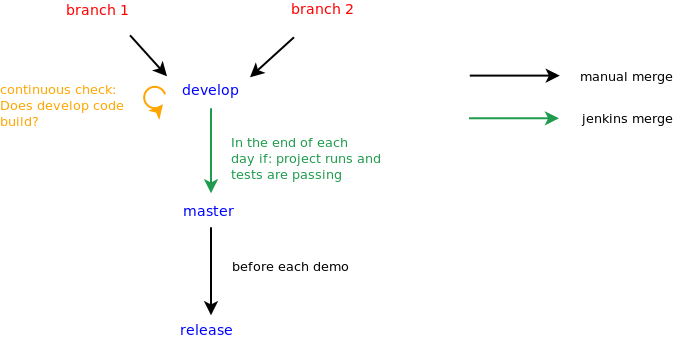
\includegraphics[scale=0.5]{frontend_workflow}
\caption{The Git workflow}\label{fig:workflow}
\end{figure}


\fig{workflow} describes our git workflow.
Each developer works on his/her own branch and merges 
the changes made into the develop branch. Jenkins is continuously
building all the code on the develop branch, so that any change that 
fails the build will be reported. The ones that have changed the code
and thus introduced a bug will be notified via E-mail about
the failed build.

On top of that, Jenkins will merge the develop code into our
master branch in the end of each day, if all tests are passing and
if the project can be build.

If you want to see the corresponding Jenkins job, that
merges the develop code into the master, go to:

\begin{myindentpar}{1cm}
\url{http://130.238.15.219:8080/job/frontend-test/}
\end{myindentpar}
\end{document}
